\documentclass{article}
\usepackage{amssymb}
\usepackage{amsmath}
\usepackage{tikz}
\usepackage{pgfplots}
\usepackage{enumitem}
\usepackage{listings}
\usepackage{color}
\usepackage{graphicx}
\usepackage{pdfpages}

\newlist{alphalist}{enumerate}{1}
\setlist[alphalist,1]{label=\textbf{\Alph*.}}

\definecolor{codegreen}{rgb}{0,0.6,0}
\definecolor{codegray}{rgb}{0.5,0.5,0.5}
\definecolor{codepurple}{rgb}{0.58,0,0.82}
\definecolor{backcolour}{rgb}{0.95,0.95,0.92}

\lstdefinestyle{mystyle}{
   backgroundcolor=\color{backcolour},
   commentstyle=\color{codegreen},
   keywordstyle=\color{magenta},
   numberstyle=\tiny\color{codegray},
   stringstyle=\color{codepurple},
   basicstyle=\footnotesize,
   breakatwhitespace=false,
   breaklines=true,
   captionpos=b,
   keepspaces=true,
   numbers=left,
   numbersep=5pt,
   showspaces=false,
   showstringspaces=false,
   showtabs=false,
   tabsize=2
}

\lstset{style=mystyle}

\begin{document}

\begin{flushleft}
  Eli Schmitter
\end{flushleft}
\section{R12.1}
\begin{enumerate}
  \item Gather requirements
  \item Use CRC cards to find classes, responsibilities, and collaborators
  \item Use UML diagrams to record class relationships.
  \item Use javadoc to document method behavior.
\end{enumerate}
\section{R12.4}
\paragraph{}
It is important to identify the object that is responsible is so you can see if the method need more methods or other classes it carry out the method.
\section{R12.5}
\begin{alphalist}
  \item aggregation
  \item inheritance
  \item inheritance
  \item neither
  \item aggregation
  \item inheritance
  \item neither
  \item neither
\end{alphalist}
\section{R12.11}
\begin{tabular}{lll|ll}
\hline
\multicolumn{5}{|l|}{Country}                         \\
\hline
\multicolumn{3}{|l|}{population} & \multicolumn{2}{l|}{} \\
\multicolumn{3}{|l|}{area} & \multicolumn{2}{l|}{} \\
\multicolumn{3}{|l|}{population density} & \multicolumn{2}{l|}{}\\
\hline
\end{tabular}
\\\\
\begin{tabular}{lll|ll}
\hline
\multicolumn{5}{|l|}{FileIn}                         \\
\hline
\multicolumn{3}{|l|}{Read} & \multicolumn{2}{l|}{} \\
\multicolumn{3}{|l|}{find the largest area} & \multicolumn{2}{l|}{} \\
\multicolumn{3}{|l|}{find the largest population} & \multicolumn{2}{l|}{}\\
\multicolumn{3}{|l|}{find the largest population density} & \multicolumn{2}{l|}{}\\
\hline
\end{tabular}
\subsection{UML}
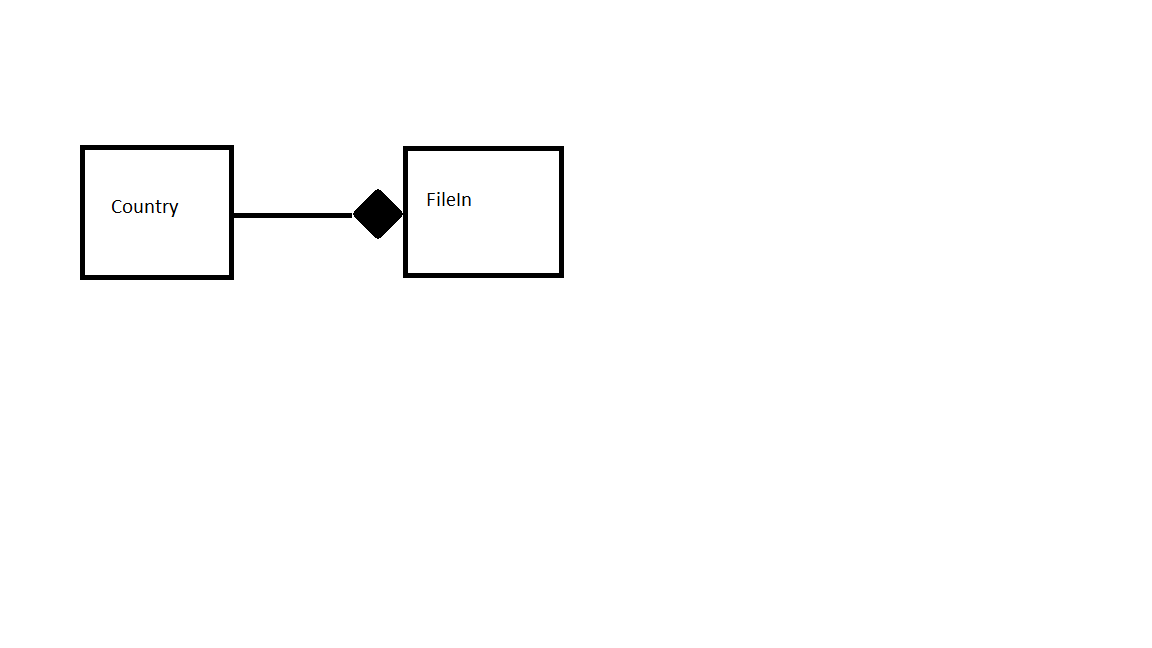
\includegraphics[height=6cm]{Untitled.png}
\subsection{Javadoc}
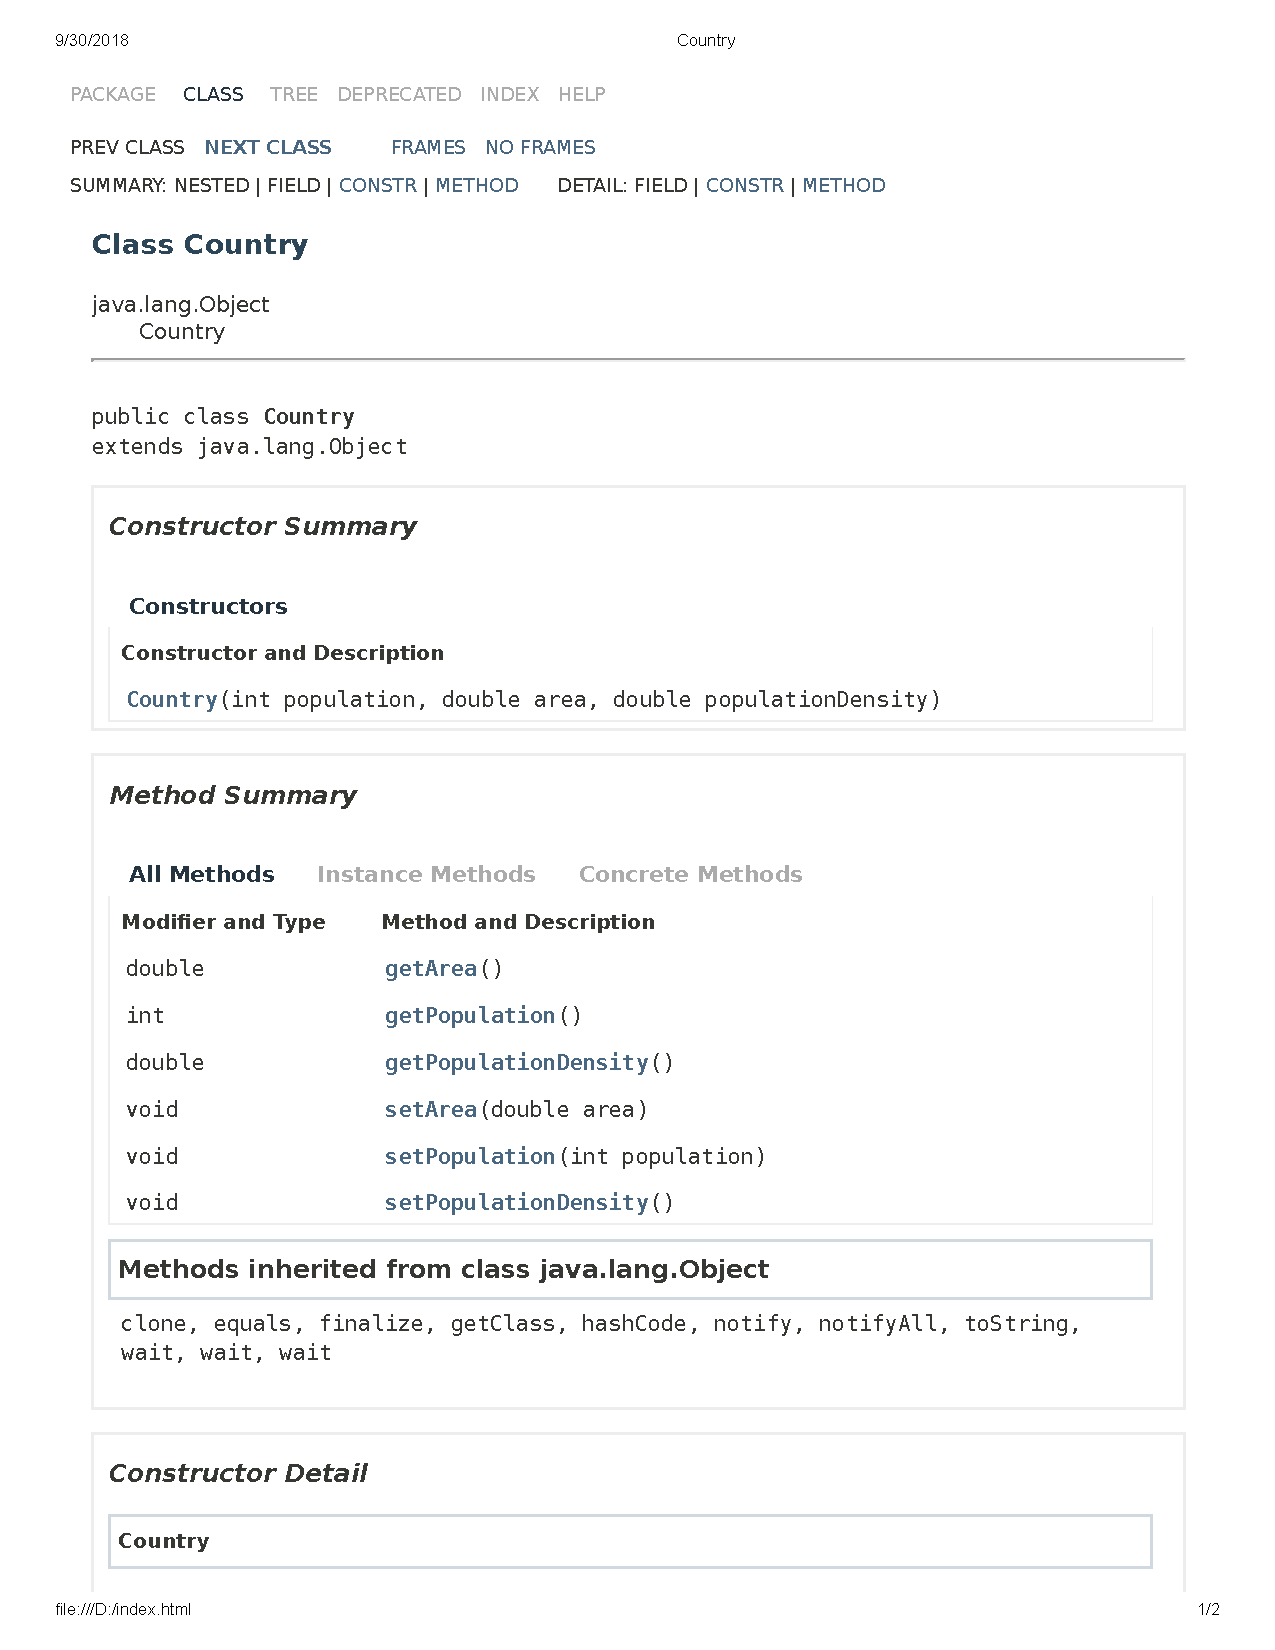
\includepdf[page={1,2}]{Country.pdf}
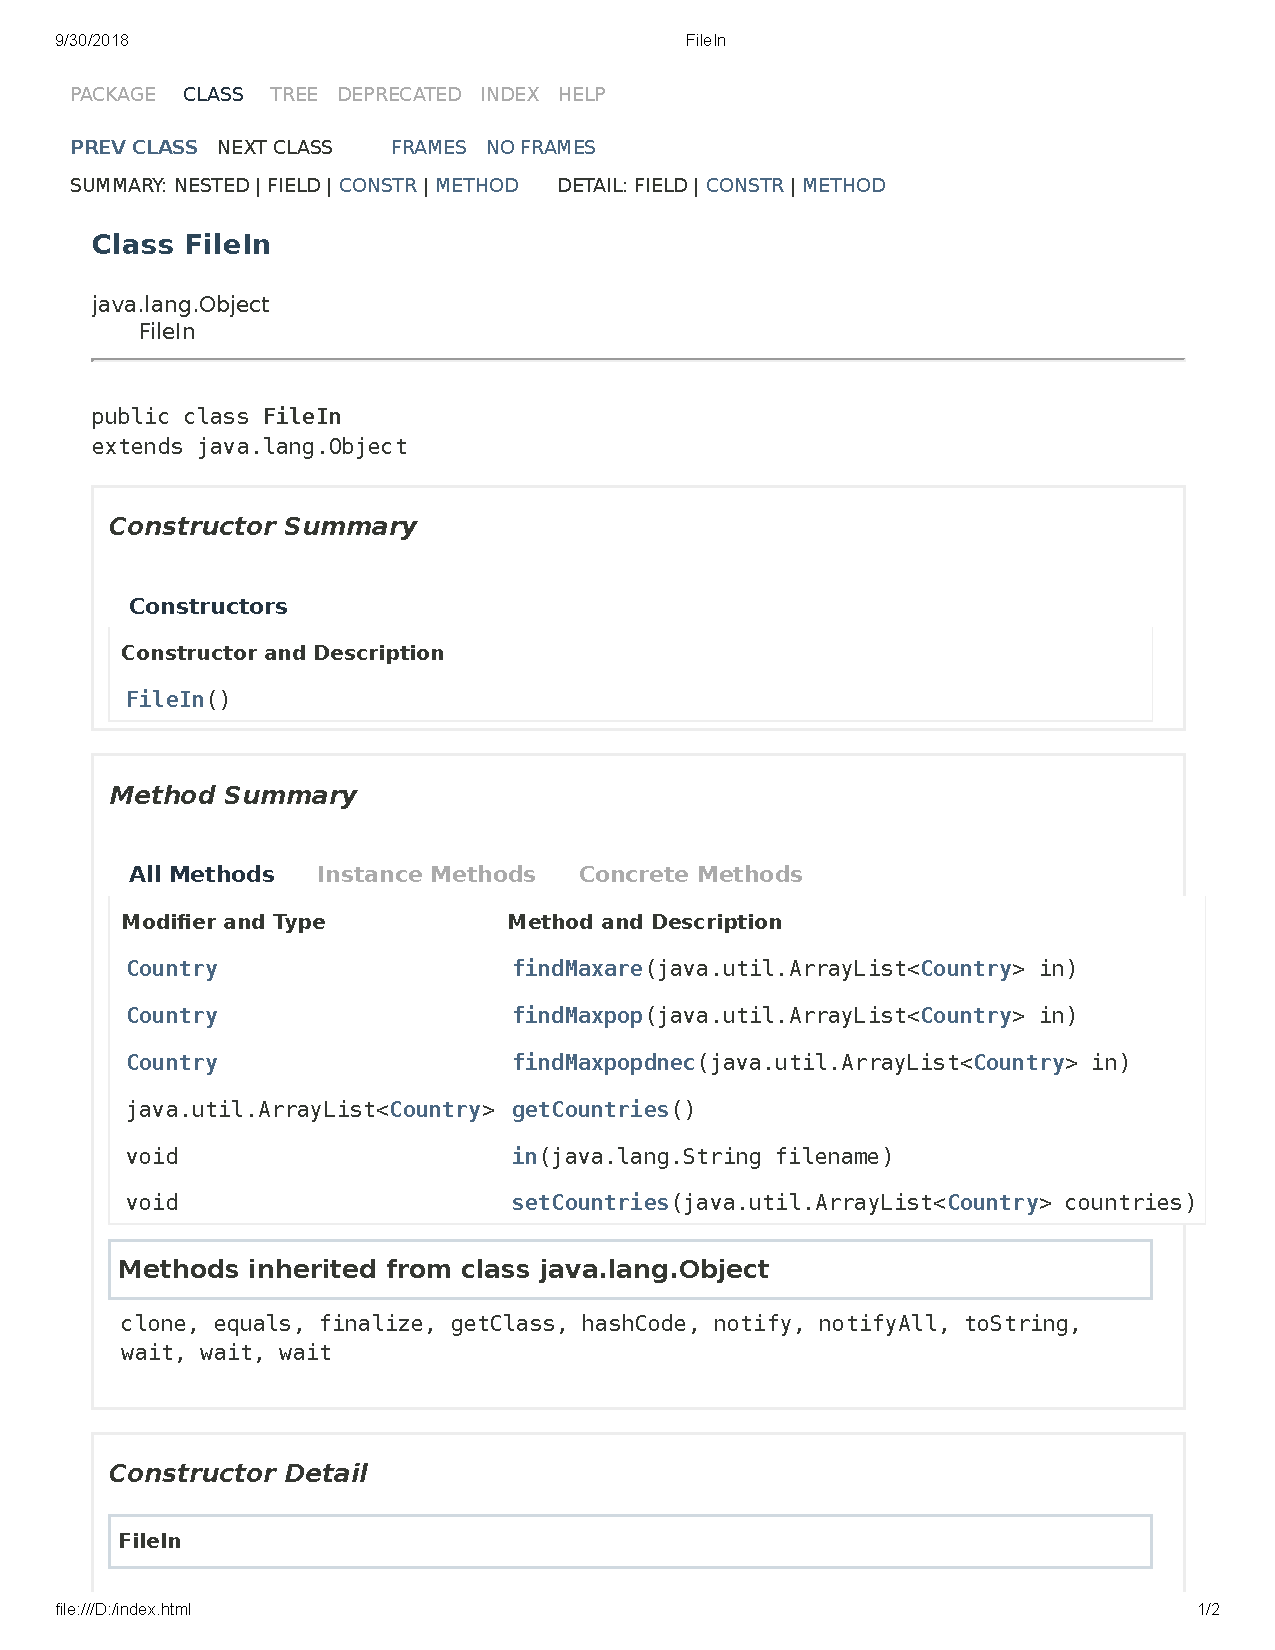
\includepdf[page={1,2}]{fileIn.pdf}
\end{document}
